%!TEX encoding=UTF-8 Unicode
\chapter{Analyzing Fine Grained Memory Traces}

\begin{itemize}
    \item \gls{Tabarnac}
        \begin{itemize}
            \item difficulty extract pertinent informations.
            \item Non interactive => user cannot explore traces
            \item 2D data structures / Threads
            \item Aspects: amount of acc, first touch, structures charactristics
        \end{itemize}
    \item \gls{Moca}
        \begin{itemize}
            \item More Generic
            \item Interactivity 
            \item 5D: Data structure, Time, Thread, CPU Locality, Memory Addresses
            \item Aspects: Sharing, Temporal patterns, Physical mapping of addresses
            \item Need “easy” way to highlight meaningful information
            \item Need a model of the trace
        \end{itemize}
    \item Contribs:
        \begin{itemize}
            \item  Moca Importer
            \item  Several fix in Framesoc / Ocelotl
            \item  Research report
            \item  Bitbucket: labbook, ongoing work
            \item  Automatic analysis: internship report
        \end{itemize}
\end{itemize}

\section{First attempt}

Modelization, meaningful agregation
Rely on Framesoc~\cite{Pagano14frameSoC} tool Ocelotl~\cite{Dosimont14Ocelotl}

\subsection{Framesoc and Ocelotl}

\begin{itemize}
    \item \gls{Framesoc}
        \begin{itemize}
            \item Generic trace representation
                \begin{itemize}
                    \item Event Producers
                    \item Event / Variables
                    \item Event Types
                    \item State
                    \item Traces DB
                \end{itemize}
            \item Multi view
            \item Possibility to filter
            \item Optimized (caches etc.)
            \item Easy to build importers
        \end{itemize}
    \item \gls{Ocelotl}~\cite{Pagano13TraceRR}
        \begin{itemize}
            \item Aggregation based on entropy
            \item Interactive aggregation / desaggregation
            \item Zoom capacity
        \end{itemize}
\end{itemize}

\subsection{Trace Description}

\begin{itemize}
    \item Producers: Addresses
    \item One trace per visu: Phy, Virt, Per threads
    \item Other info as event parameters
    \item Access = variable
    \item Artificial Mem Heirarchy: struct => Page => cache line, with tree
\end{itemize}

\subsection{Visualization}

\DB{Adapt from Moca RR}


\gls{Moca}'s output is designed to be imported inside the trace visualisation framework \gls{Framesoc} \cite{Pagano13Trace}, and to be visualised using \gls{Ocelotl} \cite{Dosimont14Trace}.
This tool uses an adaptive algorithm to aggregate data.
This algorithm returns a set of results which provides a trade-off between the information loss and the reduction of the visualisation complexity.
The user has then the possibility to move the cursor between a precise view of the trace or something more aggregated.
Moreover it provides the ability to navigate through the trace, focus on one type of event or another.

\begin{figure}[htb]
    \centering
    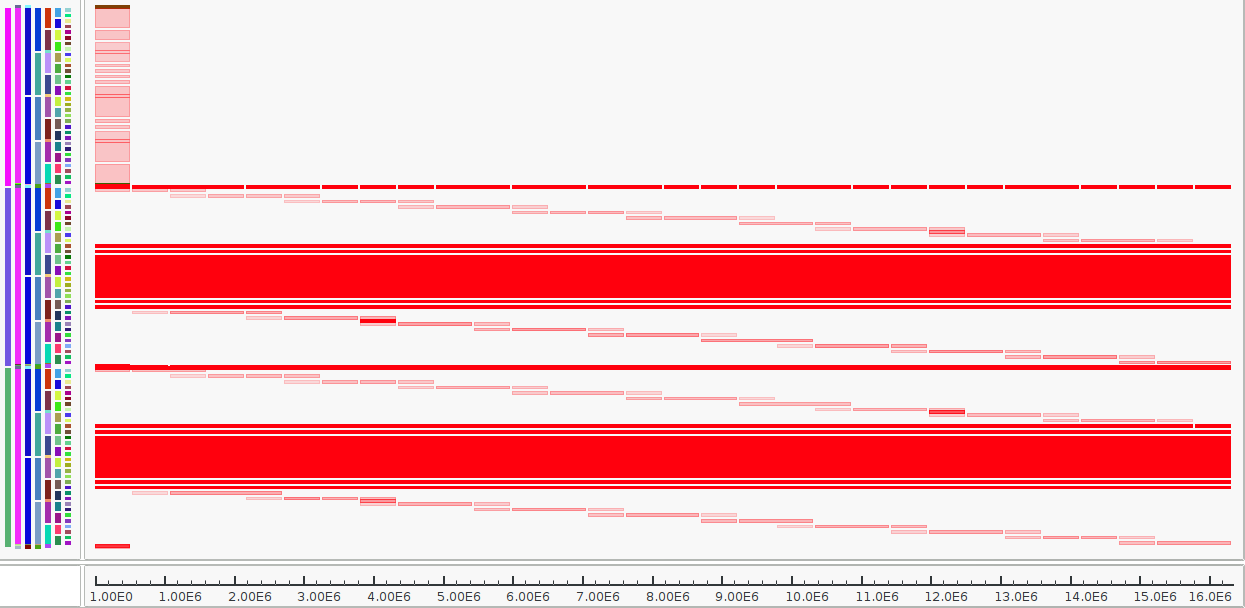
\includegraphics[width=\textwidth]{Moca-RR/multModuloThreadView.png}
    \caption{Memory-gantt view of a parallel matrix multiplication.}
    \label{fig:ocelotl-th0}
\end{figure}


We provide two different views of \gls{Moca}'s traces.
The first, is a \emph{memory gantt chart}, it shows memory usage of each threads, as we can see in \fig{ocelotl-th0}.
This view can be used to spot difference in the memory usage in terms of quantity or pattern.
The second, quite similar to HeapInfo's cartography, displays the memory addresses accessed depending on the time, as we can see in \fig{ocelotl-carto0}.
It allows the user to focus on the global memory pattern.
We provide both views for physical and virtual addresses.
Most of the time virtual addresses are recommended to have a better understanding of what the code is doing.
However, working on physical addresses can be useful for \emph{NUMA} machines to detect remote access.
We will explain how to use these views in the next section.

\begin{figure}[htb]
    \centering
    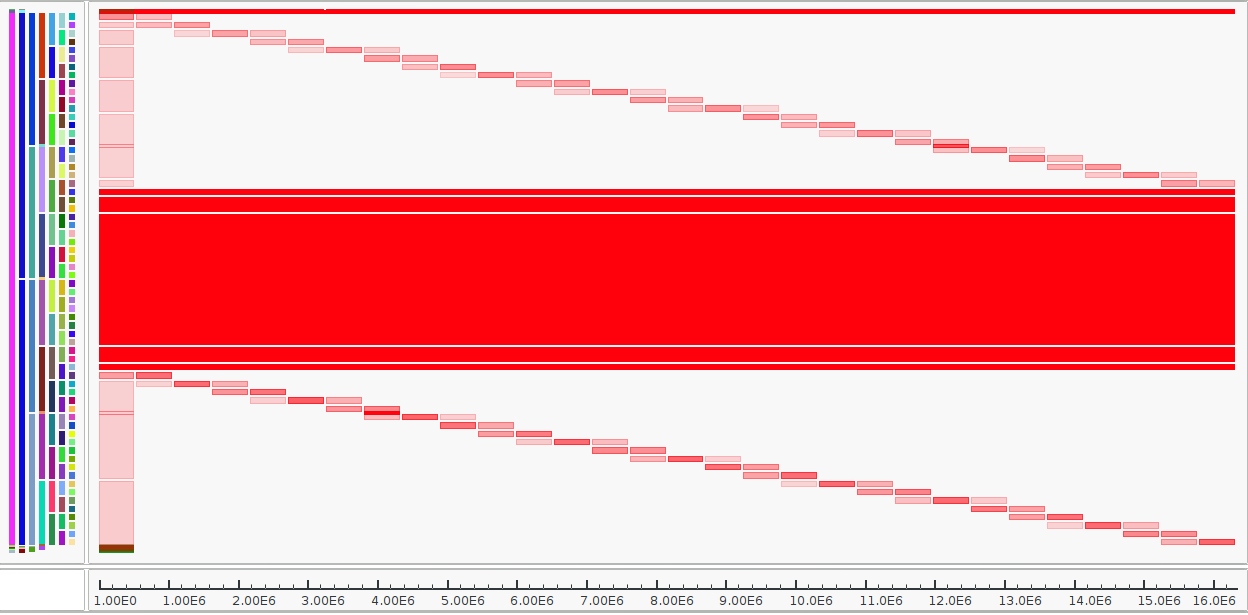
\includegraphics[width=\textwidth]{Moca-RR/multModuloCartoView.png}
    \caption{Cartography view of a parallel matrix multiplication}
    \label{fig:ocelotl-carto0}
\end{figure}

On both figures, we can notice that the memory hierarchy (on the left) is a tree.
For the first view, the top level correspond to the threads/ processes.
In figure \fig{ocelotl-th0} we can clearly identify $3$ threads.
The second level is created by merging together successive set of addresses.
Every other level is computed by cutting the previous into two or three parts.
The last level corresponds to the pages address detected by \gls{Moca}.
 Although this hierarchy is a bit artificial it shows the different parts of the memory (stack, heap, library, etc.).
Furthermore, it can be used to compute a pre aggregation which can speed \gls{Ocelotl}~up.
For the cartography view, the tree is identical, except that the first level is the second one of the memory gantt view.

\subsubsection{Example on a matrix multiplication}

\begin{algorithm}
    \caption{Naïve parallel matrix multiplication.}
    \label{alg:mat-par}
    \begin{algorithmic}
        \For{l=0; l<sz; l++}
            \For{c=myid(); c<sz; c+=NbThreads()}
                \For{k=0; k<sz; k++}
                \State Res[l][c]=A[l][k]*B[k][c]
                \EndFor
            \EndFor
        \EndFor
    \end{algorithmic}
\end{algorithm}

In this section, we show an example use of \gls{Moca}.
The studied application is a parallel matrix multiplication done by $2$ threads.
The algorithm is quite naive: a master thread initializes the matrix then creates two threads.
Each thread will compute half of the result matrix: the first will do the even index and the second the odds, which gives us the \alg{mat-par}.


If we go back to figure \fig{ocelotl-th0}, we see clearly the master/slave behavior of the threads.
While the two slave threads have a similar memory access pattern, the master threads seems to do all its access at the beginning of the execution.
Moreover it seems to access all the memory at once.
We can also see that it does less access at a time as the blocks are lighter.
From this picture, we can clearly identify two phases:
\begin{enumerate}
    \item The three threads seem to use the memory, it is the initialization phase.
    \item Only two threads are awake, they follow the same access pattern: it
        is the computational phase.
\end{enumerate}

\begin{figure}[htb]
    \centering
    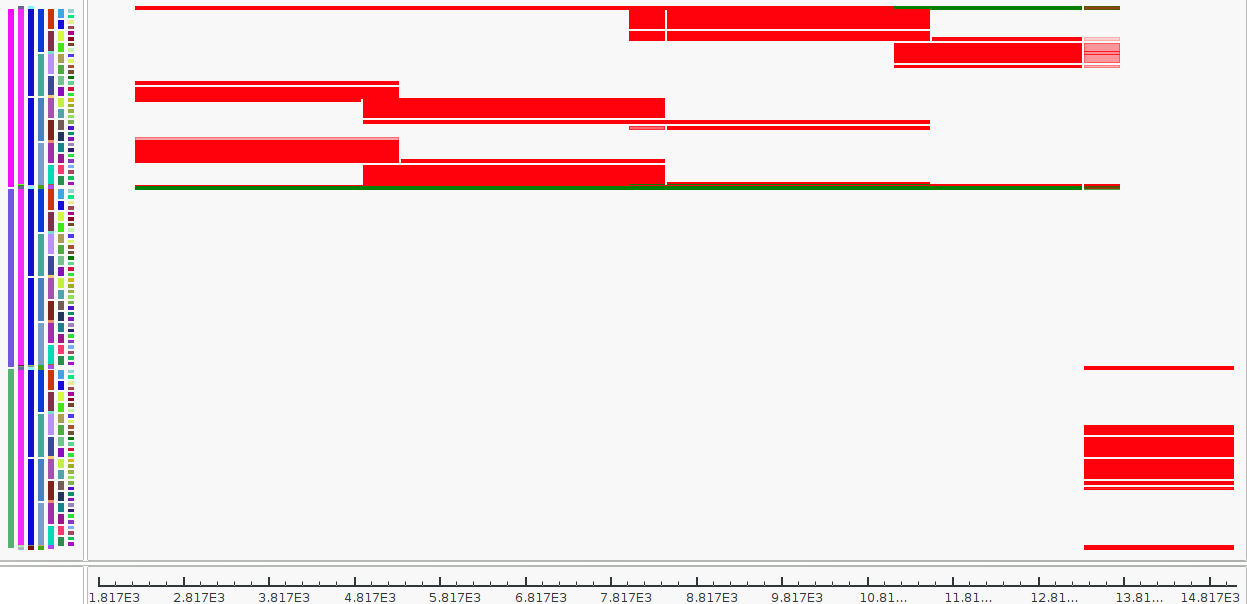
\includegraphics[width=\textwidth]{Moca-RR/multModuloThreadViewInit.png}
    \caption{Memory-gantt view of a paralell matrix multiplication,
    initialisation}
    \label{fig:ocelotl-th1}
\end{figure}

Now let's zoom on the initialisation step.
The result is shown in figure \fig{ocelotl-th1}.
We can clearly see that, contrary to what we thought on the last picture, during the initialisation phase, only the master thread is working.
We can identify a three diagonal patterns happening at the same time, it correspond to the matrix initialisation.
Moreover we see a few green access, while all the other are reds.
Here a red access mean that it is on a page used by several threads, while green is for private data.
Therefore we can see that the master thread also access to some private data.
Among these data, we can find a pid array used to wait the end of the slave threads.

The cartography view of this initialisation phase, is almost identical except that we won't be able to know which thread is responsible for the accesses.
However the global cartography view shown in figure \fig{ocelotl-carto0} gives more information.
In addition to the two execution phases, we can clearly identify three memory structures with different access patterns.
Those structures correspond to the matrices.
For the first and the third, we can see a regular diagonal access pattern which means that the matrix are accessed linearly.
As most cache optimizations such as \emph{prefetching} are designed for linear access, his is a good pattern.

\begin{figure}[htb]
    \centering
    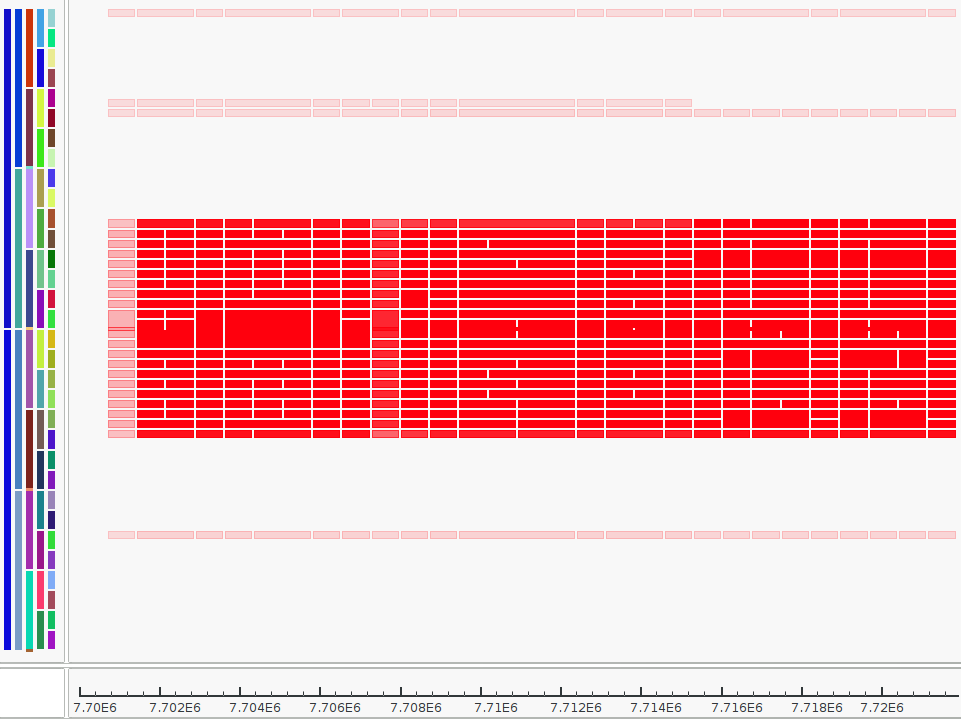
\includegraphics[width=\textwidth]{Moca-RR/multModuloCartoViewMiddle2.png}
    \caption{Cartography view of a parallel matrix multiplication, computing
    phase.}
    \label{fig:ocelotl-Carto2}
\end{figure}

By focusing on the middle of the execution and setting the aggregation to $0$, we obtain the figure \fig{ocelotl-Carto2}.
We can't identify a clear pattern on the middle matrix, however, we see that at each time slots we access more a slightly different part of the matrix (the lighter a block is, the less access it contains).
The access on this matrix seems  dense and not designed to fit in a cache.
Now, if we take a look at the algorithm \alg{mat-par}, we can explain the density of the accesses.
We go through all the matrix B while working on only one line of A.
Moreover the two threads works on two different columns at the same time, while the work on the same lines of A and Res.
Due to the representation of 2D matrix in \texttt{C}, each access on B is separated from $sz$ doubles.
Hence \gls{Ocelotl} groups almost everything in a huge chunks of access on all the matrices.
To improve this application, we should try to work on small blocks of B.
This is indeed the strategy used to compute efficient matrix multiplication.
Although this example is quite simple, it shows how \gls{Moca}'s trace can easily highlight wrong memory access patterns.

\subsection{Discussion}

\begin{itemize}
    \item  Not that interactive / too slow
    \item  Impossible to switch “aspect” of trace without reloading full trace
    \item  Hard to identify data structures
    \item  Conclusion: tool not well suited, need something more flexible
\end{itemize}

\section{Second attempt}

\begin{itemize}
    \item Exploration with R rather than full tool.
    \item Helps finding useful views
    \item R dataframes => weel design to switch point of view
    \item Work with labboks \DBm{Ref ?}
\end{itemize}

\subsection{Design}

\begin{enumerate}
    \item Parsing (csv)
    \item Retrieving mapping page => structures
    \item Creating simplified data frames
    \item Predefined plots
    \item Easily zoom  with R selection
    \item Modify plots and/or data frame
\end{enumerate}

\subsection{Results and discussion}

\begin{itemize}
    \item Small example
    \item Easy switch between views
    \item Limit: when lots of library
    \item Require that the user masters R
\end{itemize}

\section{Possible future work}

Build user friendly trace viewer based on R analysis, using R-shiny or user friendly shell on top of R.

\subsection{Generic trace visu R}

Hypothetical tool
\begin{itemize}
    \item Goal:
        \begin{itemize}
            \item More user friendly than simple R
            \item Provide default parsing and visu
            \item Can analysis any trace
            \item Enable roll back if data frame messed up without repeating parsing
        \end{itemize}
    \item Configurations
        \begin{itemize}
            \item Define mandatory arguments (trace files)
            \item R: parsing
            \item R: Default visu
        \end{itemize}
    \item Interactions:
        \begin{itemize}
            \item Do parsing
            \item Do plots
            \item See code (parsing / plot)
            \item Apply code (possibly from models)
        \end{itemize}
    \item Data frame stack
        \begin{itemize}
            \item Every modification copy the data frame
            \item Possibility to roll back on the stack
        \end{itemize}
\end{itemize}
\DB{Figure ?}

\subsection{Automatic analysis}

\DB{Voir rapport Sebastien}

\section{Discussions}

\begin{itemize}
    \item Still ongoing work
    \item Hard due to number of dimension
    \item Need meaningful way to zoom / aggregate
    \item Ocelotl main drawback: impossible to switch between aspects.
    \item Compromise: facility to interact with the trace, semantic of the interaction
    \item Possible solution: build abstraction on top of R
\end{itemize}

% vim: et si sta lbr  sw=4 ts=4 spelllang=en_us
